\documentclass{report}
\usepackage[left=2cm,right=2cm,top=2cm,bottom=2cm,bindingoffset=0cm]{geometry}
\usepackage[utf8x]{inputenc}
\usepackage[english,russian]{babel}
\usepackage{amsfonts}
\usepackage{amsmath}
\usepackage{mathtools}

\usepackage{graphicx}
\graphicspath{{pictures/}}
\DeclareGraphicsExtensions{.pdf,.png,.jpg}

\begin{document}
\LARGE{ \textbf {Лекция №9}}\\
\Large{ \textbf {}}\\

Синхронный двуступеньчатый D-триггер с запрещабщими связями.\\

Принцип построения такой же как JK.\\
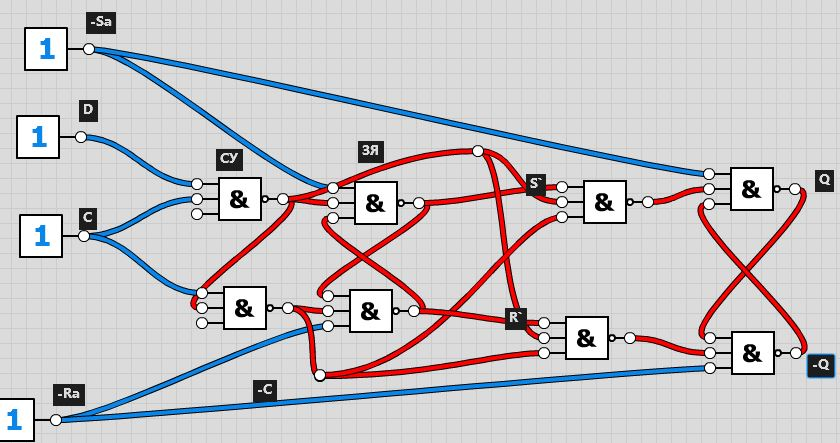
\includegraphics[width=\linewidth*3/4]{34}\\
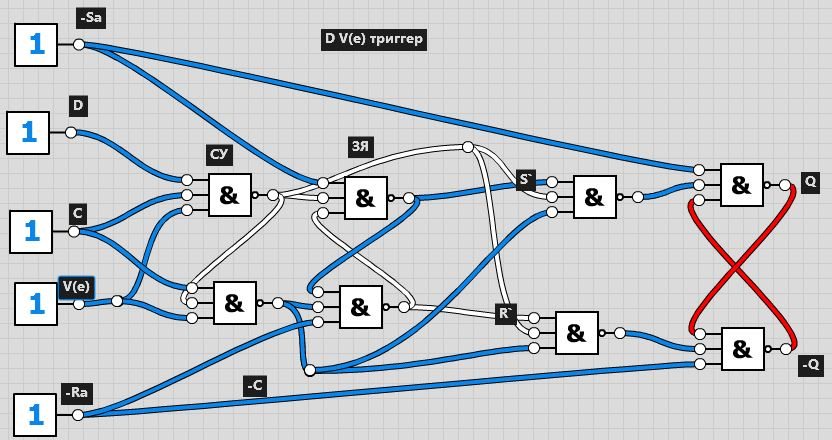
\includegraphics[width=\linewidth*3/4]{35}\\
Почему нельзя использовать односторонний D-триггер в качестве счетного триггера со статическим управлением записью ? С динамическим управлением можно.\\

\textbf{RS-триггер с разнополярным управлением.}
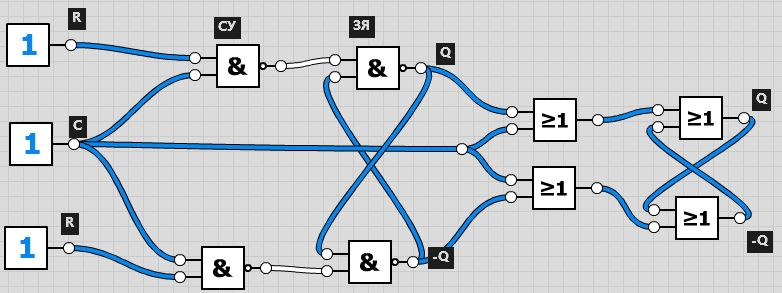
\includegraphics[width=\linewidth*3/4]{36}\\
$t_{u} => 6t^*_{zaderSR}$\\
$t_{n} => 3t^*_{zaderSR}$\\
$T => 6t^*_{zaderSR} $\\
$f_{max} = \frac{1}{ 6t^*_{zaderSR}} $\\



\textbf{Синхронные триггеры с динамическим управлением записью.}
Они управляются перепадом из нуля в единицу - передний фронт. Из единицы в нуль -1/0 задний фронт.
Информация в триггер записывается только в момент действия перепада синхро сигнала.\\

\textbf{Синхронный D-триггер с динамическим управлением записью.}\\
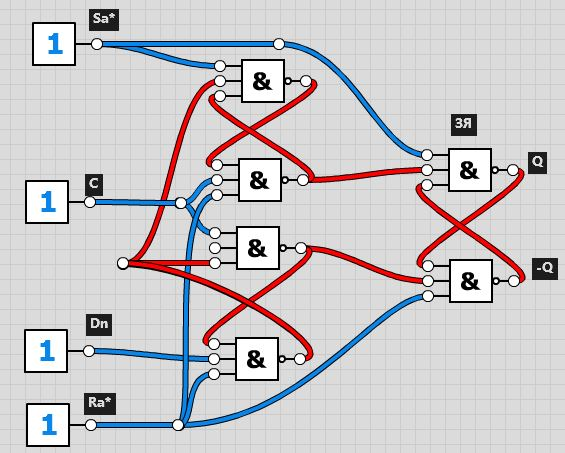
\includegraphics[width=\linewidth*3/4]{37}\\

Триггер управляется передним фронтом, то есть перепадом из 0 в 1 .
Схема состоит из основого триггера - ЗЯ то что справа.
И двух вспомагательных ЛЭ 1,2,3,4 которые служат для записи 1 и 0 в основной триггер.
То есть Q и не Q являются  выходными сигналами триггера в целом.

Sa = 1 , Ra = 1\\
При С=0 - Q2 = Q3 = 1 - режим хранения.
$Q_4 = \overline {Q_3 * D *R = -D }  $ \\
$Q_1 = \overline{ Q_4 * Q_2 *S = -D }  $ \\
При с= 0 один из триггеров всегда находится в неправльном состоянии. Оба выходных сигнала равны 1.
При С = 1, такое состояние исчезает.\\
D =  0

При с = 1 и D = 1
Q2 = 0. Ноль с выхода ЛЭ1 блокирует логические элементы 1 и 3.

Запись информации станет возможна только тогда, когда С опять станет равным 0.

Одноступеньчатый синхронный D-триггер можно использовать в качестве счетного триггера.


\textbf{Функциональные узлы ЭЛМ. }
Узел - функциональная часть ЭВм предназначенная для выполнения операций надо словом или частью слова.
Слово - совокупность бит.

Класисификация узлов \\
По назначению
\begin{enumerate}
  \item Шифраторы - дешифраторы
  \item Мультиплексторы - де
  \item Регистры
  \item Счетчики
  \item Сумматоры
  \item Схемы сравнения кодов
\end{enumerate}
По принципу логического функционирования:\\
Комбинационные, накапливающего типа.\\

\textbf{Функциональные узлы накапливающего типа.}\\
\textbf{Регистр}\\
Функциональный узел - предназначенный для ввода, хранения, преобразования, вывода двоичного слова или его части.\\
\begin{itemize}
\item Некоторые микрооперации можно разделить на 4 группы. \\
\item Связанные с приемом слова, установка в 0,1. Прием слова в прямом или обратном коде.\\
\item Выдача слова в прямом или обратном коде.\\
\item Выполнение поразрядных логических операций.\\
\item Сдвиг слов влево, вправо. На то или оное число разрядов.
\item Преобразование последовательного ввода в паралелльный и обратно.


\end{itemize}
По способу ввода и вывода информации регистры различают на \\
\begin{itemize}
\item Паралелльные - просто регистр памяти.
Ввода и вывод выполняется одновременно по всем разрядам. Каждый разряд передается по своей отдельной цепи.
\item Последовательные - регистры сдвига.
Разряды слова передаются последовательно во времени и пространстве, как при вводе так и выводе.
\item Паралелльно-последовательные. Кроме того могут выполнять взаимные преобразования последовательных входов в парралельные и обратно.
\end{itemize}

По способу представленния на выходе\\
Парафазные-
И прямое значени выводится и инверсное.Требуется 2 линии связи.\\
Однофазные
Либо только прямой выход, либо только инверсный.\\

Паралелльные регисты\\
Выполняют операции хранения, записи и выдачи чисел. Число триггеров в регистре равно ислу разрядов в слове.\\

Регистр на RS триггерах.\\
Если ПЧ = 0, R = 0 =>Q=0\\
ПЧ = 1, R = 0 => Q = xi\\
Происходит запись только единичных значений, нулевые значачния не меняются. \\
Запись в такой регистр требует обязательной установки в 0(весь его)\\
Однофазный по входу, парафазный по выходу.\\

Парафазный регистр на RS триггерах

 регистр на D триггерах\\
ВПК = 1 , ВОК = 0

ВПК = 0 , ВОК = 1

ВПК =  ВОК = 0

ВПК =  ВОК = 1

СХЕМЫ ВЕЗДЕ !!!!!
\end{document}
